\subsection{Алгоритмы имитации отжига.
Проблема возможности потери лучшего решения.
Способы распараллеливания алгоритма имитации отжига.}

Алгоритм имитации отжига основан на аналогии с физическим процессом отжига металлов. На каждом шаге с вероятностью, зависящей от текущей «температуры» $T$, допускается переход в состояние с худшим значением целевой функции:
\[
P(X^k \to X^{k+1}) = 
\begin{cases} 
1, & \Delta F \leq 0 \\ 
\exp\left(-\frac{\Delta F}{T}\right), & \Delta F > 0 
\end{cases}
\]
где $\Delta F = F(X') - F(X)$. 

\subsubsection*{Законы понижения температуры}
Температура $T$ снижается в соответствии с выбранным законом, что влияет на баланс между исследованием пространства решений и эксплуатацией текущего минимума. Основные подходы:
\begin{itemize}
    \item \textbf{Закон Больцмана}:  
    \[
    T(i) = \frac{T_0}{\ln(1+i)},
    \]
    где $i$ — номер итерации. Медленное снижение, подходит для задач с большим пространством поиска.

    \item \textbf{Закон Коши}:  
    \[
    T(i) = \frac{T_0}{1+i}.
    \]
    Более быстрое снижение температуры, уменьшает время вычислений.

    \item 
	\[
		T(i) = T_0\cdot\frac{\ln{1+i}}{1+i}.
    \]

    \end{itemize}

\subsubsection*{Проблема потери лучшего решения}
При вероятностном принятии решений существует риск потери наилучшего найденного решения, особенно при неоптимальном выборе закона охлаждения:
\begin{itemize}
    \item \textbf{Быстрое снижение $T$} (Коши, экспоненциальный закон) — риск застревания в локальном минимуме.
    \item \textbf{Медленное снижение $T$} (Больцмана) — увеличение времени вычислений и шанс «перепрыгивания» лучшего решения.
\end{itemize}
Стратегии предотвращения:
\begin{itemize}
    \item Сохранение лучшего решения в отдельной переменной.
    \item Использование адаптивных законов (динамический закон) для управления $T$ в зависимости от истории улучшений.
    \item Введение механизма «отката» к лучшему решению при длительном отсутствии прогресса.
\end{itemize}

\subsubsection*{Способы распараллеливания}
Распараллеливание алгоритма может быть реализовано следующими способами:

\begin{enumerate}
    \item \textbf{Асинхронная схема} (рис. \ref{fig:async}): 
    \begin{itemize}
        \item Каждый процессор работает с локальной копией решения.
        \item Периодически обменивается лучшими решениями с другими узлами.
        \item Не требует синхронизации между итерациями.
    \end{itemize}
    
    \begin{figure}[h]
        \centering
        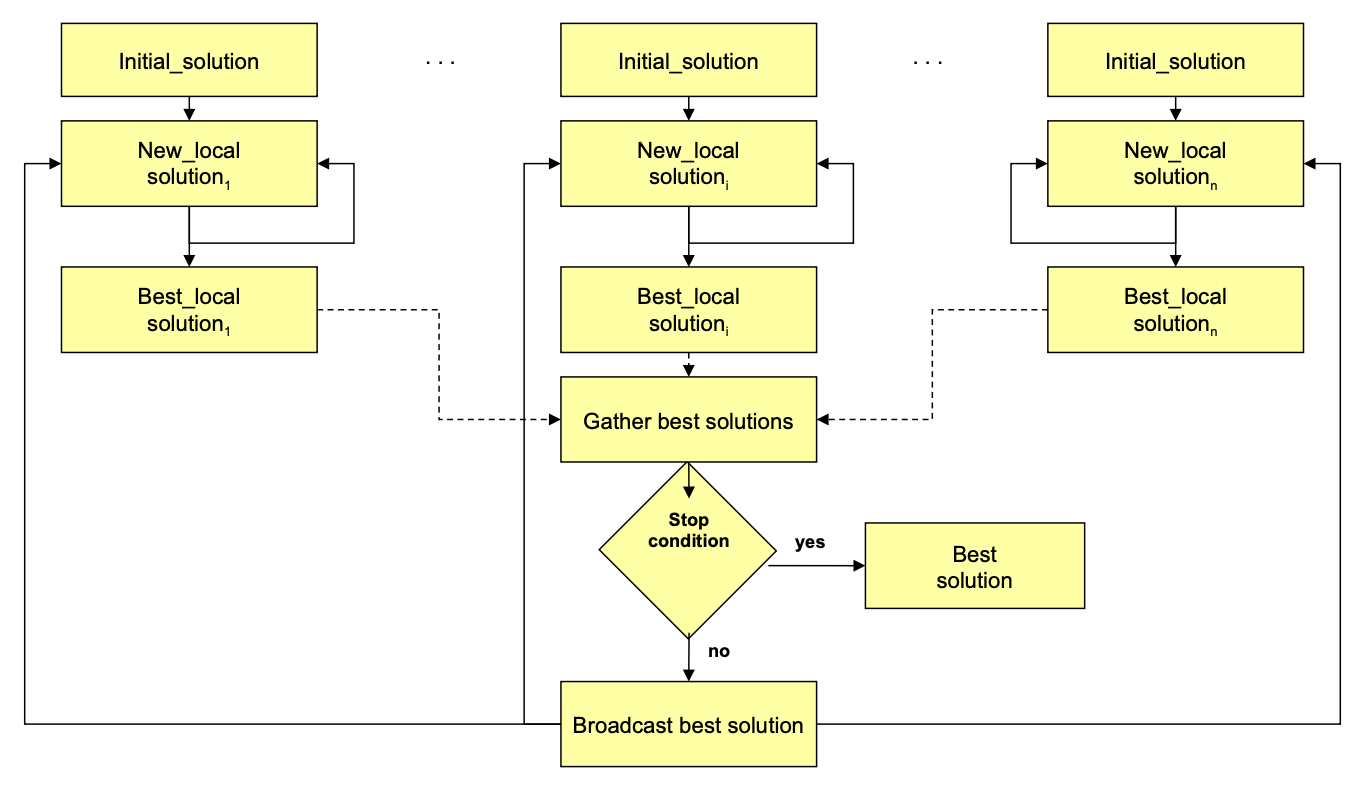
\includegraphics[width=0.8\textwidth]{pics/IOpar1.png}
        \caption{Схема асинхронного параллельного алгоритма имитации отжига}
        \label{fig:async}
    \end{figure}

    \item \textbf{Синхронная схема} (рис. \ref{fig:sync}):
    \begin{itemize}
        \item Процессоры синхронизируются на каждой итерации.
        \item Координатор собирает решения, выбирает глобально лучшее.
        \item Обеспечивает детерминированность, но увеличивает накладные расходы.
    \end{itemize}
    
    \begin{figure}[h]
        \centering
        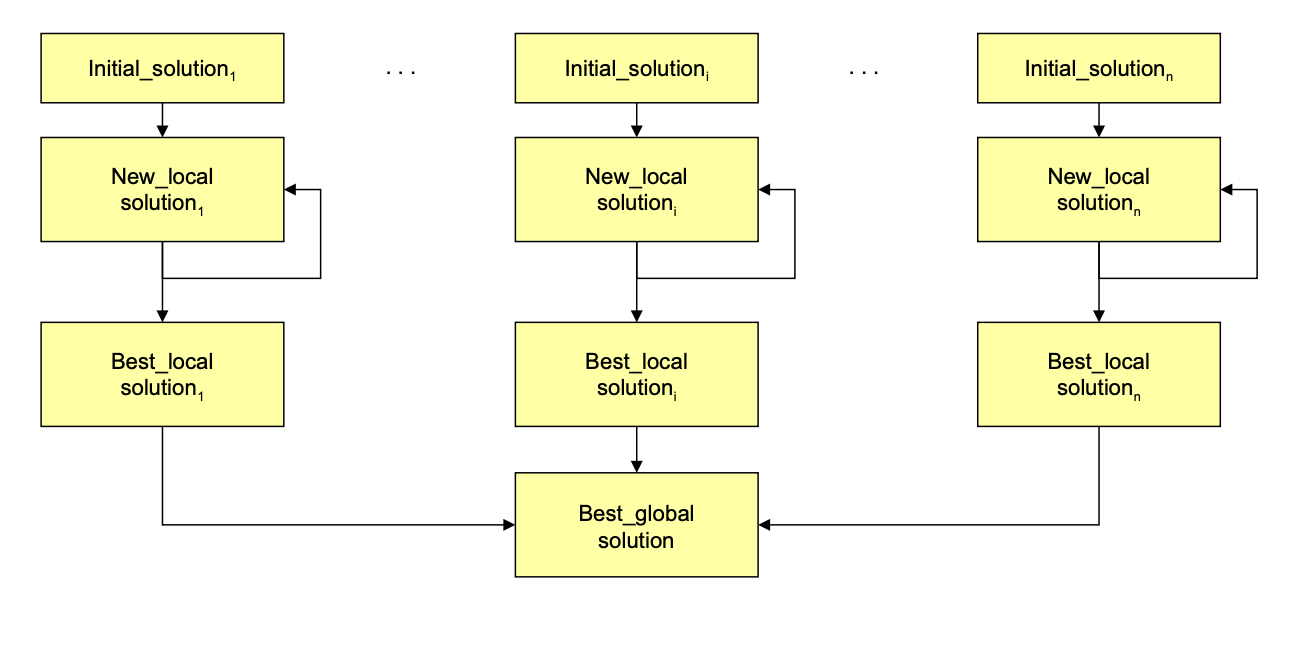
\includegraphics[width=0.8\textwidth]{pics/IOpar2.png}
        \caption{Схема синхронного параллельного алгоритма с координатором}
        \label{fig:sync}
    \end{figure}
\end{enumerate}

Дополнительные подходы:
\begin{itemize}
    \item \textbf{Декомпозиция целевой функции} — параллельное вычисление независимых компонент.
    \item \textbf{Разбиение пространства решений} — распределение областей поиска между узлами.
    \item \textbf{Гибридные стратегии} — комбинация распараллеливания с динамическим управлением $T$.
\end{itemize}

Материалы, основываясь на которых написан билет~\cite{kostenko_lectures}
